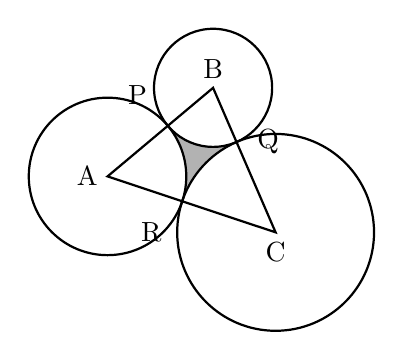
\begin{tikzpicture}[scale=1]

    % Define radii proportional to the actual problem measurements (AP=4, PB=3, RC=5) 
    % Scaled down by a factor of 4 for drawing purposes
    \def\rA{1.0}
    \def\rB{0.75}
    \def\rC{1.25}

    % Define centers using precise mathematical placement so the circles touch perfectly.
    \coordinate (A) at (0, 0);
    
    % Place B at an angle of 40 degrees from A
    \coordinate (B) at ({1.75*cos(40)}, {1.75*sin(40)});
    
    % Angle for C is calculated so that distance BC is exactly rB + rC = 2.0
    \coordinate (C) at ({2.25*cos(-18.41186)}, {2.25*sin(-18.41186)});

    % 1. Shade the exact region between the circles using a clipping scope
    \begin{scope}
        % Clip everything to the bounds of the triangle ABC
        \clip (A) -- (B) -- (C) -- cycle;
        % Fill the clipped triangle with gray
        \fill[gray!60] (A) -- (B) -- (C) -- cycle;
        % "Erase" the corners by filling the circles with white
        \fill[white] (A) circle (\rA);
        \fill[white] (B) circle (\rB);
        \fill[white] (C) circle (\rC);
    \end{scope}

    % 2. Draw the circles
    \draw[thick] (A) circle (\rA);
    \draw[thick] (B) circle (\rB);
    \draw[thick] (C) circle (\rC);

    % 3. Draw the triangle connecting the centers
    \draw[thick] (A) -- (B) -- (C) -- cycle;

    % 4. Define and place the intersection (touch) points exactly along the paths
    \path (A) -- (B) coordinate[pos=0.5714] (P); % Ratio: rA / (rA + rB)
    \path (B) -- (C) coordinate[pos=0.3750] (Q); % Ratio: rB / (rB + rC)
    \path (A) -- (C) coordinate[pos=0.4444] (R); % Ratio: rA / (rA + rC)

    % 5. Add text labels exactly as in the image
    \node[left] at (A) {A};
    \node[above] at (B) {B};
    \node[below] at (C) {C};

    % Shifted the labels P, Q, and R further away to prevent overlapping
    \node[above left, xshift=-4pt, yshift=4pt] at (P) {P};
    \node[right, xshift=4pt] at (Q) {Q};
    \node[below left, xshift=-4pt, yshift=-4pt] at (R) {R};

\end{tikzpicture}